\chapter{Studies of inconsistency indexes for incomplete matrices}
\label{sec:studiesOfInconsistencyIndexesForIncompleteMatrices}

The presented inconsistency indexes have been tested utilizing the Monte Carlo method. Their aim was to select those indexes which will give reliable results for incomplete matrices. Therefore, it was decided that the measure of the indexes' quality would be a \textit{relative error} (expressed as a percentage), which took into account the value of the index for a full, inconsistent matrix and the value of the index for the same matrix after partial decomposition. To be sure that the results were fair, all indexes were tested on the same set of matrices. The different sizes of the matrices, the levels of incompleteness and the levels of inconsistency were taken into account. Then, in order to compare the indexes easily and to select the best ones, the results were averaged using the arithmetic mean. While building the algorithm to solve the problem (Kazibudzki, 2017) was used.


\section{Algorithm}
\subsection{Steps of the algorithm}
\textbf{Procedure steps:}
\begin{enumerate}
\item Randomly generate a vector $w=[w_{1},...,w_{n}]$ and a consistent \textit{PCM matrix} associated with it $PCM=\left(m_{ij}\right)$, where $m_{ij}=\frac{w_{i}}{w_{j}}$.
\item Disrupt the matrix by multiplying its elements (excluding the diagonal) by the value of $d$, randomly selected from the range $\left(\frac{1}{x},x\right)$.
\item Replace values $m_{ij}$, where $i<j$ by values $m_{ji}$.

\item Calculate values of index with all methods for the created matrix.

\item Remove some values from the matrix by removing some of values. The level of incompleteness should be $g$\%.

\item Calculate the values of inconsistencies by all methods for the decomposed matrix.

\item Calculate the relative error for each index.

\item Repeat steps 1 to 10 $X_{1}$ times.

\item Calculate the average relative error for each inconsistency index for the \textit{PCM matrix}.

\item Repeat steps 1 to 10 $X_{2}$ times.

\item Calculate the average relative error for each index by averaging the values obtained in step 9.

\end{enumerate}


\subsection{Details of algorithm}
The above algorithm was carried out for values $X_{1}=100$, $X_{2}=100$. Tests were started for values d in the range $\left(1.1,1.2,...,4\right)$ and then the results were averaged. It means that the average relative error of one index was calculated on the basis of 4000 matrices, each of which decomposed randomly 100 times. It gave together 400000 tests how good the index was. 
\\

In addition, tests were carried out for various sizes of matrices.\\
\textbf{The results are divided into two parts:}
\begin{enumerate}
  \item A constant degree of incompleteness, different size of the matrix.
  \item Different degrees of incompleteness, constant size of the matrix.
\end{enumerate}

The aim of such a division is to pay attention to how the inconsistency indexes behave when the size of the matrix and the degree of incompleteness are changing. The results of the research are presented below.


\section{Implementation}

\subsection{Development environment}
Tests of indexes have been developed in R language which is appropriate for nuimerical calculations. It contains dozens of functions which support operations on matrixes and vectors. Integrated development environment (IDE) called \testit{RStudio} has been used during implementation. This tool allows to create own packages which contains not only code but also documentation and information about licence and author. Package named \textit{indexesForIncomplete} has been created. The most important part of this package is file \textit{indexes.R} which performs calculations necessery to test indexes. \testit{RStudio} supports programmer's work by syntax highlighting, built-in console, easy documentation searching and many others. The program is available on common operating systems. Before using \testit{RStudio} one have to install \textIt{R} programming language.  
% https://pbiecek.gitbooks.io/przewodnik/content/Programowanie/podstawy/jak_zainstalowac_R.html
% https://cran.r-project.org/
% https://www.rstudio.com/products/RStudio/
\begin{figure}[h]
\centerline{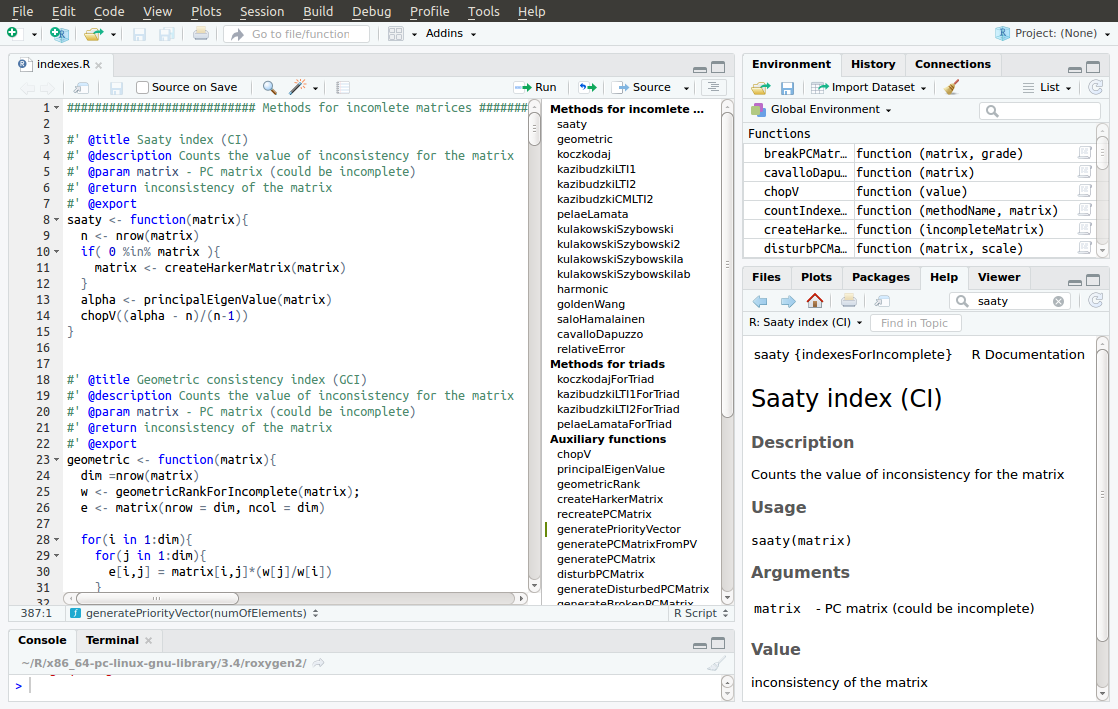
\includegraphics[width=\textwidth]{images/rstudio.png}}
\caption{Program \textit{RStudio}}
\label{fig:rstudio}
\end{figure}


\subsection{Implementation of tests of inconsistency indexes}
Implementation of tests inconsistency indexes consists of two steps:
\begin{enumerate}
  \item Implementation of functions which calculates inconsistency indexes for given matrix (full or incomplete).
  \item Implementation of tests which studies indexes for different matrixes and collects all results of these tests. 
\end{enumerate}

\subsubsection{Implementation of inconsistency indexes}
Sixteen functions which calculate inconsistency indexes using methods described in chapter 3. The functions have been wroten in such a way that allows handle both full and incomplete matrixes. One have not taken account of wrong matrixes, it means nonreciprocal or inconsistent PC matrixes. Each of these function has only one parameter - \textif{PC matrix}. Exceptions are two methods implementing Kulakowski and Szybowski index which additionally take parameters $\alpha, \beta$. The result of each function is value of inconsistency index. The functions have been extended by comments which informs about name of index related to given function, parameters and returned value. It allows to easily read and modify the code. Several examples of functions are presented below.

\begin{figure}[h]
\centerline{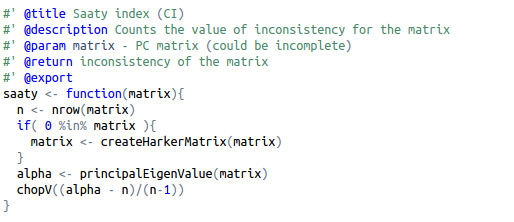
\includegraphics[scale=0.75]{images/kod1.png}}
\caption{The implementation of \textit{Saaty} index}
\label{fig:rstudio}
\end{figure}

\begin{figure}[h]
\centerline{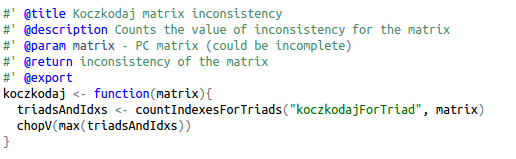
\includegraphics[scale=0.75]{images/kod2.png}}
\caption{The implementation of \textit{Koczkodaj} index}
\label{fig:rstudio}
\end{figure}

\begin{figure}[h]
\centerline{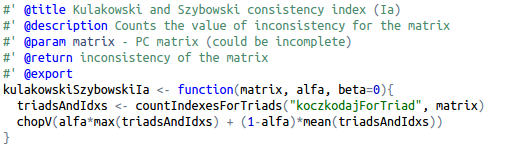
\includegraphics[scale=0.75]{images/kod3.png}}
\caption{The implementation of \textit{Kulakowski and Szybowski} index}
\label{fig:rstudio}
\end{figure}

\begin{figure}[h]
\centerline{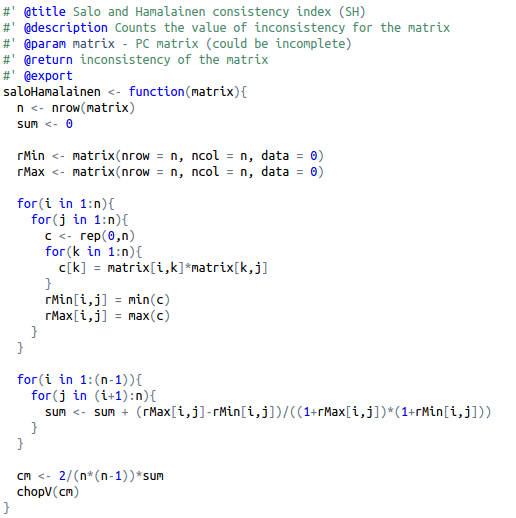
\includegraphics[scale=0.75]{images/kod4.png}}
\caption{The implementation of \textit{Salo and Hamalainen} index}
\label{fig:rstudio}
\end{figure}
It is worth drawing attention to function which is called within the functions intended for indexes based on triads. This function generates triads from a matrix and next returns inconsistency for each o them. However, the way to calculate inconsistency for one triad depends on first function parameter. It informs about function name that calculates inconsistency of a triad specified method.

\begin{figure}[h]
\centerline{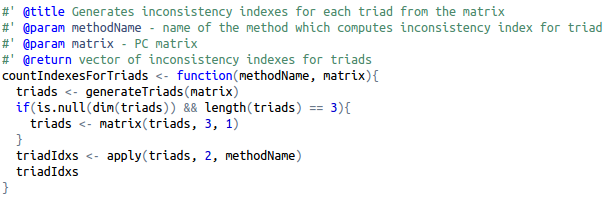
\includegraphics[scale=0.75]{images/kod5.png}}
\caption{The implementation of method \textit{countIndexesForTriads}, which calculates inconsistency for each triad of a specified matrix}
\label{fig:rstudio}
\end{figure}


\subsubsection{Implementation of tests}
In the second step functions, which calculate the quality of the indexes for incomplete matrices, have been created. Functions, which generate specified matrixes, plays an important role. PC matrixes are created depending on size, the level of inconsistency and the degree of incompleteness.

\begin{figure}[h]
\centerline{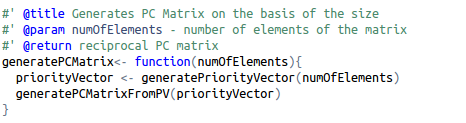
\includegraphics[scale=0.75]{images/kod11.png}}
\caption{The implementation of function \textit{generatePCMatrix} which generates the PC matrix depending on matrix size}
\label{fig:rstudio}
\end{figure}

\begin{figure}[h]
\centerline{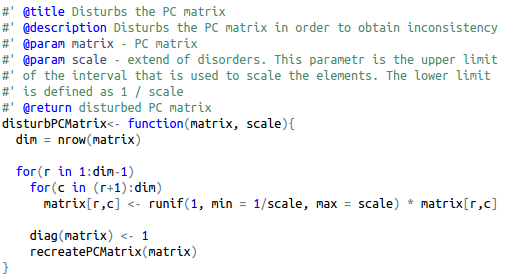
\includegraphics[scale=0.75]{images/kod12.png}}
\caption{The implementation of function \textit{disturbPCMatrix} which disturbs the PC matrix regarding inconsistency depending on given level of inconsistency}
\label{fig:rstudio}
\end{figure}

\begin{figure}[h]
\centerline{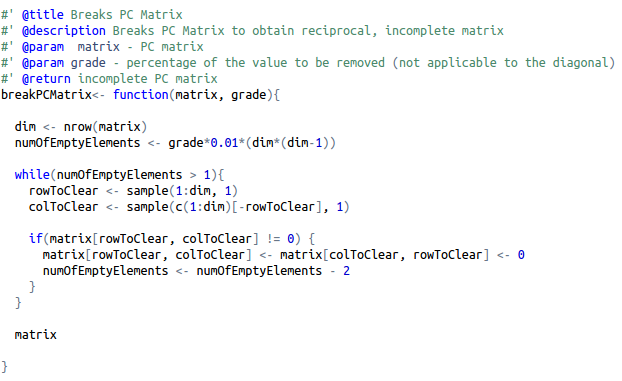
\includegraphics[scale=0.73]{images/kod13.png}}
\caption{The implementation of function \textit{breakPCMatrix} which breaks up the PC matrix regarding incompleteness depending on given degree of incompleteness}
\label{fig:rstudio}
\end{figure}

The last part of functions relates testing how big relative error occurs for inconsistency indexes after deleting some values. To begin with functions, which test one index. They consider matrix size, the level of inconsistency, the degree of incompleteness and the number of attempts which are performed for given matrix.

\begin{figure}[h]
\centerline{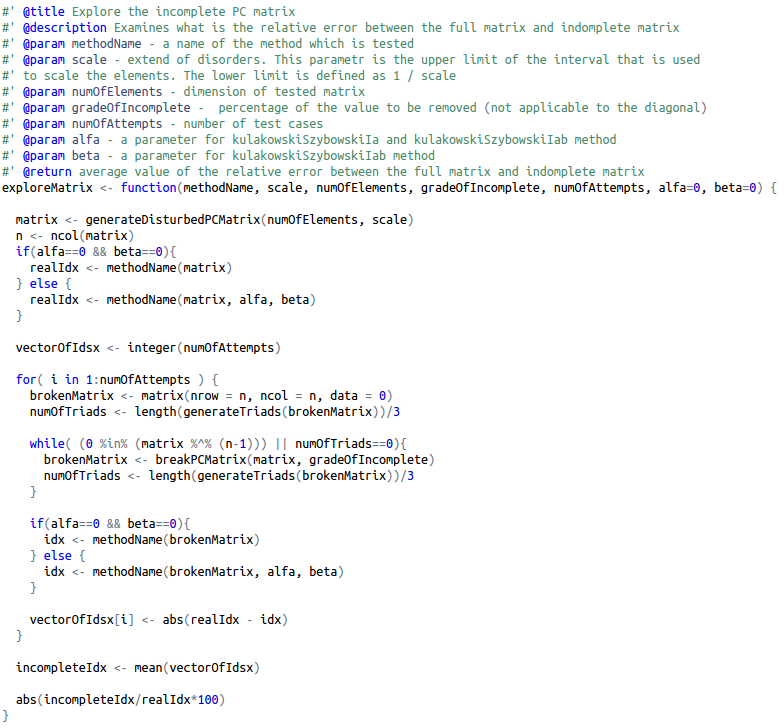
\includegraphics[scale=0.58]{images/kod21.png}}
\caption{The implementation of function \textit{exploreMatrix} which tests given inconsistency index}
\label{fig:rstudio}
\end{figure}

Then functions, which perform tests for each indexes, has been developed basing on the same matrixes. In that the set of matrixes , on which indexes go, is common. Thus, results are reliable and each index is considered the same way.

\begin{figure}[h]
\centerline{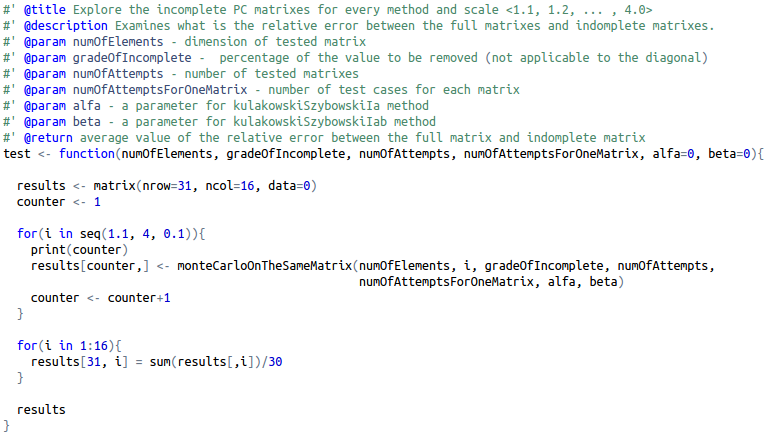
\includegraphics[scale=0.58]{images/kod22.png}}
\caption{The implementation of function \textit{test} which tests all indexes regarding given matrix size and the degree of incompleteness}
\label{fig:rstudio}
\end{figure}


\subsection{Documentation}
Comments in code have been used to generating documentation. the package \textit{roxygen2} has been made for this purpose. It has allowed to easy review code and know the functions./
Exemplary portions of the documentation are presented below.

\begin{figure}[h]
\centerline{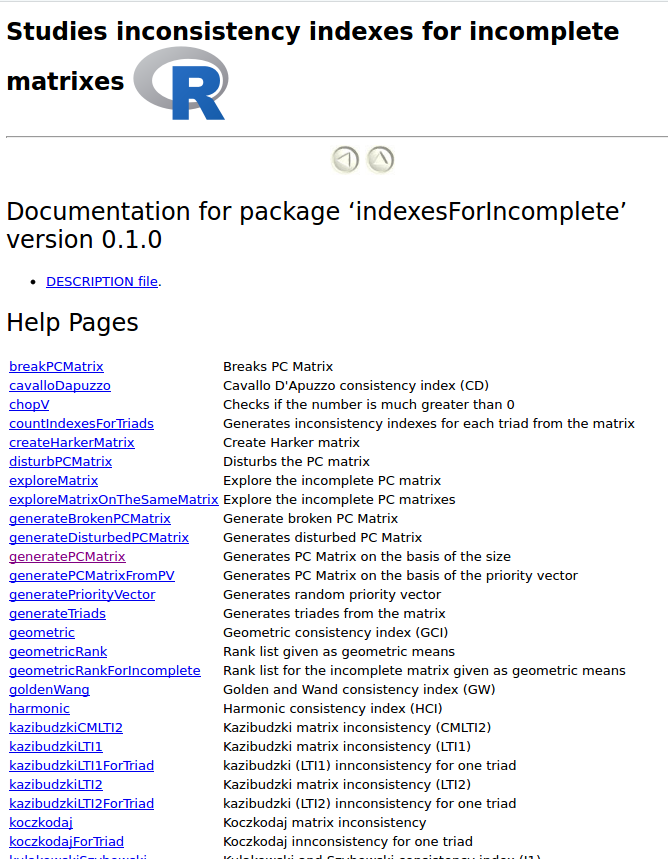
\includegraphics[scale=0.58]{images/kod31.png}}
\caption{The portion of the documentation: general view}
\label{fig:rstudio}
\end{figure}

\begin{figure}[h]
\centerline{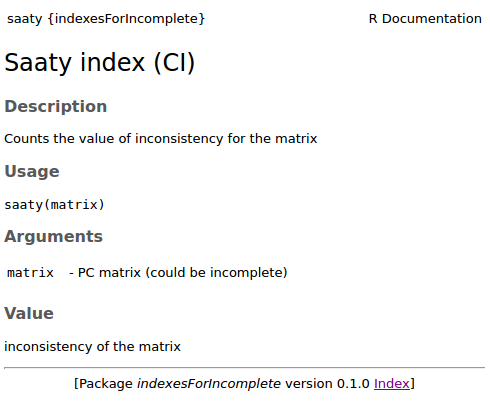
\includegraphics[scale=0.58]{images/kod32.png}}
\caption{The portion of the documentation: function \textit{saaty}}
\label{fig:rstudio}
\end{figure}

\begin{figure}[h]
\centerline{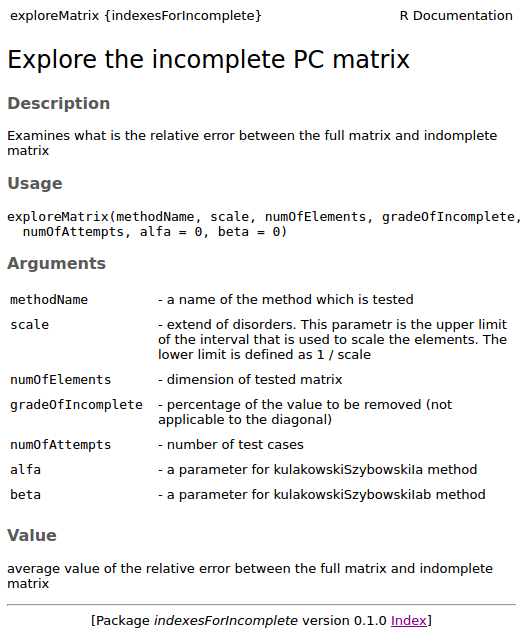
\includegraphics[scale=0.58]{images/kod33.png}}
\caption{The portion of the documentation: function \textit{exploreMatrix}}
\label{fig:rstudio}
\end{figure}